\section{Технический проект}
\subsection{Общая характеристика организации решения задачи}

Необходимо спроектировать и разработать корпоративный портал учета рабочего времени сотрудников. Разрабатываемая программная система предназначена для предоставления комплексного инструмента управления временем, который позволит сотрудникам и менеджерам эффективно отслеживать и управлять временем, затраченным на проекты и задачи.

Основной принцип работы системы заключается в управлении проектами и задачами, а также в учете рабочего времени с помощью таймшитов.

Ключевым компонентом программной системы является база данных для хранения информации о пользователях, проектах, задачах и таймшитах. База данных будет обеспечивать надежное хранение данных и быстрый доступ к ним для выполнения всех операций.

Пользовательский интерфейс будет реализован в виде web-страницы, написанной на языке разметки HTML с применением JS для обработки событий и CSS для описания стилей элементов управления.

Целью разработки данной программной системы является создание эффективного инструмента управления временем в корпоративной среде, который поможет повысить продуктивность сотрудников и оптимизировать процессы проектного управления, способствуя развитию и росту компании.

\subsection{Обоснование выбора технологии проектирования}

Используемые для создания программно-информационной системы языки и технологии отвечают современным практикам разработки, позволяют достичь высокой производительности и отказоустойчивости программы. В частности, связка HTML + CSS позволяет быстро разработать удобные и функциональные пользовательские интерфейсы, а наличие значительного количества фреймворков и библиотек для JS существенно сокращают время, затрачиваемое на разработку функциональной части интерфейса, при этом не причиняя ущерба качеству финального продукта. 

\subsubsection{Описание используемых технологий и языков программирования}

В процессе разработки интерфейса web-сайта использовались следующие языки программирования и программные средства: HTML5, JavaScript, С\# (Razor), CSS.

\subsubsection{Язык разметки HTML5}

HTML5 (HyperText Markup Language, version 5) - это последняя версия стандарта HTML, используемого для создания и структурирования web-страниц и web-приложений. HTML5 представляет собой мощный инструмент для создания современных и интерактивных web-приложений, обеспечивая разработчикам широкий набор возможностей для создания привлекательного и функционального контента в Интернете.

\subsubsection{Языки программирования и фреймворки}

\paragraph{Язык программирования JavaScript}

JavaScript - это высокоуровневый, интерпретируемый язык программирования, который применяется в web-разработке для создания интерактивных элементов на веб-страницах. Он является одним из основных инструментов фронтенд-разработки вместе с HTML и CSS. JS используется для добавления динамического поведения на страницы, обработки событий пользователя, взаимодействия с веб-серверами (через AJAX) и т.д.

\paragraph{Фреймворк Razor для языка программирования C\#}
Razor - это фреймворк, разработанный компанией Microsoft, который используется в ASP.NET для создания динамических web-страниц. Он позволяет разработчикам внедрять код C\# и VB.NET непосредственно в HTML-разметку страницы, что облегчает создание и обслуживание web-приложений. Фреймворк Razor предоставляет мощные средства для работы с данными, логикой и представлениями в веб-приложениях, а также способы для организации кода и повторного использования компонентов интерфейса.

\subsection{Компоненты web-сайта}
Все компоненты web-сайта, реализованного на фреймворке Razor могут принадлежать одной из следующих разновидностей:
\begin{itemize}
\item Частичное представление
\item Представление
\item Классы и шаблоны Razor
\item Разметка Razor
\end{itemize}
Для корректного отображения пользовательского интерфейса, все компоненты любой из этих разновидностей должны лежать в папке Pages или её подпапках. Это гарантирует удобство, простоту и скорость доступа от одного компонента к любому другому компоненту.
Диаграмма компонентов представлена на рисунке ~\ref{fig:comp}

\begin{figure}[H]
	\centering
	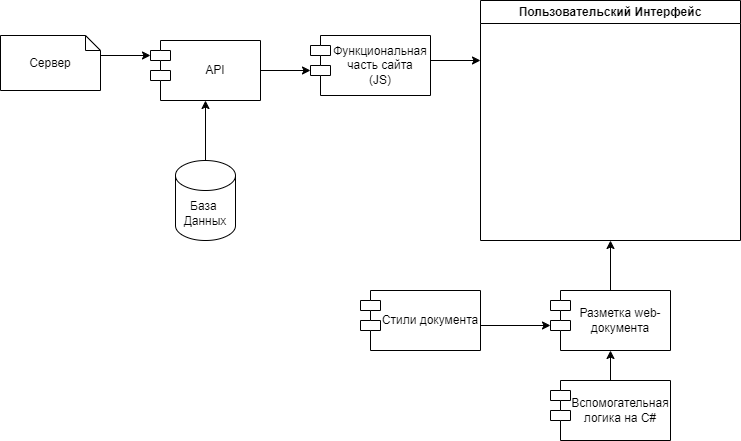
\includegraphics[width=1\linewidth]{images/comp}
	\caption{}
	\label{fig:comp}
\end{figure}

\subsection{Логика клиентской части}
Функциональная часть web-страницы выполнена на языках JavsScript и C\#. Код на JavaScript отвечает за обработку событий и взаимодействие с сервером через API, а код на C\# - за переключение между страницами и компонентами Razor.

\subsubsection{Обработка событий и сообщений от сервера на JS}
Глобально код на JavaScript  можно разделить на две категории: код, выполняющий обработку событий, и код, взаимодействующий с сервером. В более узком плане, код делится по зонам ответственности: класс для работы со страницей авторизации, класс для работы со страницей просмотра и класс для работы со страницей редактирования. Каждая зона ответственности вынесена в отдельный файл; каждый файл внутри логически делится на зоны категорий посредством группирования методов (перечисляются сначала функции для работы с сервером, потом функции для работы с клиентскими событиями, в конце файла идут общие функции, необходимые для построения взаимосвязей между предыдущими группами функций и обработки событий, не предполагающих участия сервера и/или пользователя). Для взаимодействия с сервером (отправка запросов, получение информации) использовалась методология AJAX. Обработка пользовательских событий (ввод информации в текстовые поля, нажатия на кнопки и т.д.) была реализована на "<чистом"> JS (без использования JQuery) с целью экономии ресурсов.
  
\subsubsection{Логика переключения компонентов Razor на С\#}
Логика переключения компонентов Razor реализуется посредством создания контроллера для каждой web-страницы, html-разметка которой расположена в папке "Pages". Контроллер принимает в качестве входных параметров и передаёт на связанную с ним страницу переменные, а также обрабатывает содержимое непосредственно самой web-страницы. Связать URL-адрес страницы и вызов контроллера (т.н. "<назначить странице URL">) можно в основном файле с кодом фреймворка Razor - app.cs через метод "Map()", принимающий на вход URL-адрес, контроллер и необязательные дополнительные параметры.

\subsection{Проектирование пользовательского интерфейса}
На основании требований к пользовательскому интерфейсу, представленных в пункте 2.3.2 технического задания, был разработан графический интерфейс web-сайта. Для создания пользовательского интерфейса используется HTML-разметка с иерархией компонентов Razor Pages.

На рисунке ~\ref{fig:inter3} представлен макет интерфейса формы авторизации. Макет содержит следующие элементы:
\begin{enumerate}
\item Поле ввода логина
\item Поле ввода пароля
\item Кнопка авторизации на портале
\end{enumerate}

\begin{figure}[H]
	\centering
	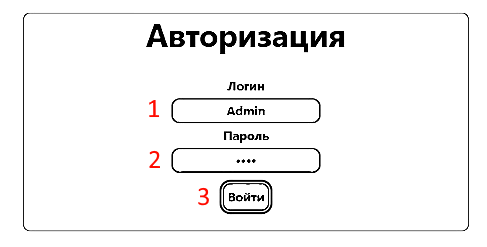
\includegraphics[width=0.5\linewidth]{images/inter3}
	\caption{Макет интерфейса формы авторизации}
	\label{fig:inter3}
\end{figure}

На рисунке ~\ref{fig:inter1} представлен макет интерфейса окна редактирования. Макет содержит следующие элементы:
\begin{enumerate}
	\item Вкладка переключения на окно редактирования
	\item Вкладка переключения на окно просмотра
	\item Кнопка добавления новой записи
	\item Кнопка изменения выбранной записи
	\item Кнопка удаления выбранной записи
	\item Таблица с интерактивными (доступными для выбора по клику правой кнопкой мыши) записями
\end{enumerate}

\begin{figure}[H]
	\centering
	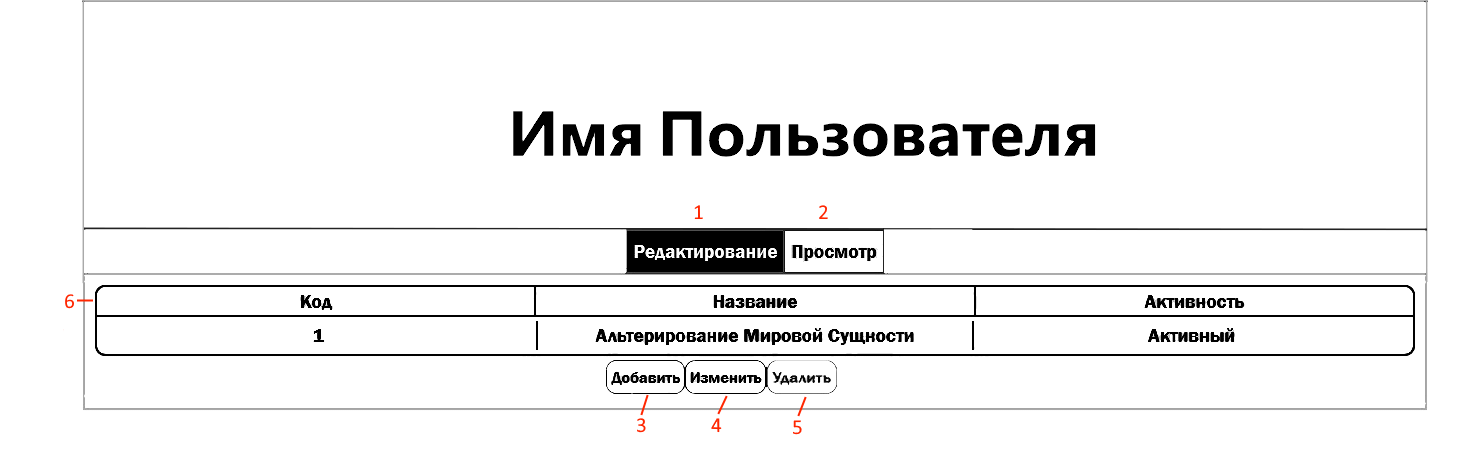
\includegraphics[width=1\linewidth]{images/inter1}
	\caption{Макет интерфейса окна редактирования}
	\label{fig:inter1}
\end{figure}

На рисунке ~\ref{fig:inter2} представлен макет интерфейса окна просмотра. Макет содержит следующие элементы:
\begin{enumerate}
	\item Вкладка переключения на окно редактирования
	\item Вкладка переключения на окно просмотра
	\item Кнопка применения фильтрации по дате
	\item Кнопка сброса фильтрации по дате
	\item Поле ввода даты нижней границы фильтрации
	\item Поле ввода даты верхней границы фильтрации
	\item Таблица с результатами фильтрации или информацией обо всех проводках текущего пользователя
\end{enumerate}

\begin{figure}[H]
	\centering
	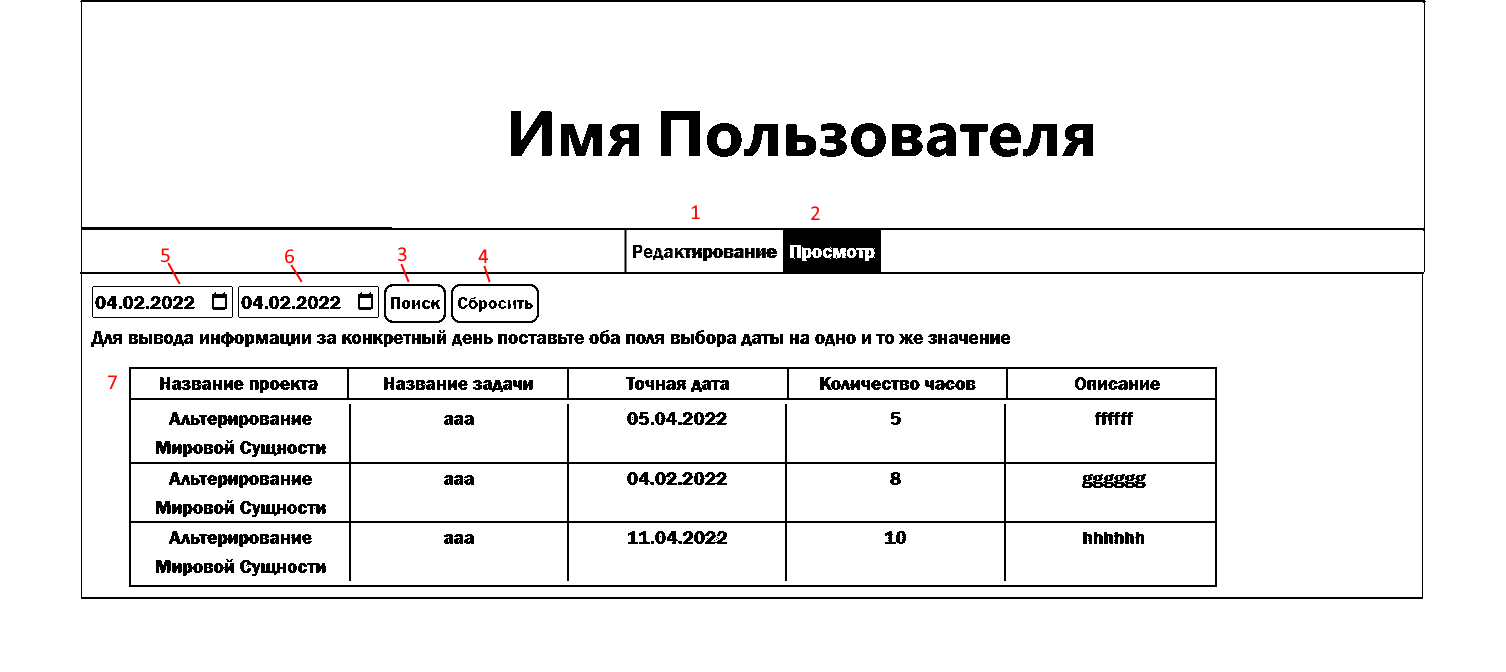
\includegraphics[width=1\linewidth]{images/inter2}
	\caption{Макет интерфейса окна просмотра}
	\label{fig:inter2}
\end{figure}